\documentclass[final,onefignum,onetabnum]{siamart190516}

%% ------------------------------------------------------------------
%% Code used in examples, needed to reproduce 
%% ------------------------------------------------------------------
%% Used for \set, used in an example below
\usepackage{braket,amsfonts}

%% Used in table example below
\usepackage{array, mathtools}

%% Used in table and figure examples below
\usepackage[caption=false]{subfig}
%% Used for papers with subtables created with the subfig package
\captionsetup[subtable]{position=bottom}
\captionsetup[table]{position=bottom}

%% Used for PgfPlots example, shown in the "Figures" section below.
\usepackage{pgfplots}

%% Used for creating new theorem and remark environments
\newsiamthm{claim}{Claim}
\newsiamremark{remark}{Remark}
\newsiamremark{hypothesis}{Hypothesis}
\crefname{hypothesis}{Hypothesis}{Hypotheses}

%% Algorithm style, could alternatively use algpseudocode
\usepackage{algorithmic}

%% For figures
\usepackage{graphicx,epstopdf}

%% For referencing line numbers
\Crefname{ALC@unique}{Line}{Lines}

%% For creating math operators
\usepackage{amsopn}
\DeclareMathOperator{\Range}{Range}

%% ------------------------------------------------------------------
%% Macros for in-document examples. These are not meant to reused for
%% SIAM journal papers.
%% ------------------------------------------------------------------
\usepackage{xspace}
\usepackage{bold-extra}
\usepackage[most]{tcolorbox}
\newcommand{\BibTeX}{{\scshape Bib}\TeX\xspace}
\newcounter{example}
\colorlet{texcscolor}{blue!50!black}
\colorlet{texemcolor}{red!70!black}
\colorlet{texpreamble}{red!70!black}
\colorlet{codebackground}{black!25!white!25}

\newcommand\bs{\symbol{'134}} % print backslash in typewriter OT1/T1
\newcommand{\preamble}[2][\small]{\textcolor{texpreamble}{#1\texttt{#2 \emph{\% <- Preamble}}}}

\lstdefinestyle{siamlatex}{%
  style=tcblatex,
  texcsstyle=*\color{texcscolor},
  texcsstyle=[2]\color{texemcolor},
  keywordstyle=[2]\color{texemcolor},
  moretexcs={cref,Cref,maketitle,mathcal,text,headers,email,url},
}

\tcbset{%
  colframe=black!75!white!75,
  coltitle=white,
  colback=codebackground, % bottom/left side
  colbacklower=white, % top/right side
  fonttitle=\bfseries,
  arc=0pt,outer arc=0pt,
  top=1pt,bottom=1pt,left=1mm,right=1mm,middle=1mm,boxsep=1mm,
  leftrule=0.3mm,rightrule=0.3mm,toprule=0.3mm,bottomrule=0.3mm,
  listing options={style=siamlatex}
}

\newtcblisting[use counter=example]{example}[2][]{%
  title={Example~\thetcbcounter: #2},#1}

\newtcbinputlisting[use counter=example]{\examplefile}[3][]{%
  title={Example~\thetcbcounter: #2},listing file={#3},#1}

\DeclareTotalTCBox{\code}{ v O{} }
{ %fontupper=\ttfamily\color{texemcolor},
  fontupper=\ttfamily\color{black},
  nobeforeafter,
  tcbox raise base,
  colback=codebackground,colframe=white,
  top=0pt,bottom=0pt,left=0mm,right=0mm,
  leftrule=0pt,rightrule=0pt,toprule=0mm,bottomrule=0mm,
  boxsep=0.5mm,
  #2}{#1}

% Stretch the pages
\patchcmd\newpage{\vfil}{}{}{}
\flushbottom

%% ------------------------------------------------------------------
%% End of macros for in-document examples. 
%% ------------------------------------------------------------------

%% ------------------------------------------------------------------
%% HEADING INFORMATION
%% ------------------------------------------------------------------
\begin{tcbverbatimwrite}{tmp_\jobname_header.tex}
\title{Recovering sparse DFT on missing signals via interior point method\thanks{Submitted to the editors DATE.
\funding{Funding information goes here.}}}

\author{Wei Kuang \thanks{University of Chicago, (\email{ddoe@imag.com}).}
\and Others \thanks{Department of Applied Math, Fictional University, Boise, ID (\email{ptfrank@fictional.edu}, \email{jesmith@fictional.edu}).}
\and others still \footnotemark[3]}

% Custom SIAM macro to insert headers
\headers{Recovering sparse DFT on missing signals via interior point method}
\end{tcbverbatimwrite}
\input{tmp_\jobname_header.tex}

% Optional: Set up PDF title and authors
\ifpdf
\hypersetup{ pdftitle={Guide to Using  SIAM'S \LaTeX\ Style} }
\fi

%% ------------------------------------------------------------------
%% END HEADING INFORMATION
%% ------------------------------------------------------------------

%% ------------------------------------------------------------------
%% MAIN Document
%% ------------------------------------------------------------------
\begin{document}
\maketitle

%% ------------------------------------------------------------------
%% ABSTRACT
%% ------------------------------------------------------------------
\begin{tcbverbatimwrite}{tmp_\jobname_abstract.tex}
\begin{abstract}
We present a method of identifying the sparsity of Discrete Fourier transform (DFT) when the signal is noisy. In particular, we consider the case where signal has some missing values. The conjugate structure of DFT makes the optimization in complex field difficult, so we transfer the problem to LASSO in real field. We introduce how to apply interior point method to solve LASSO. Besides, the orthogonal structure of inverse Discrete Fourier transform (IDFT) allows us to greatly reduced the storage. Also the operations of computing Newton direction is linear in problem size. Thus, our method is practical and scalable. 
\end{abstract}

\begin{keywords}
  \LaTeX, \BibTeX, SIAM Journals, Documentation 
\end{keywords}

\begin{AMS}
  00A20 
\end{AMS}
\end{tcbverbatimwrite}
\input{tmp_\jobname_abstract.tex}
%% ------------------------------------------------------------------
%% END HEADER
%% ------------------------------------------------------------------
\section{Introduction}
The Discrete Fourier Transform (DFT) transfers signal from the time domain to the frequency domain, thus revealing the information of spectrum. It plays important roles in many applications, such as audio and video processing, GPS, medical imaging and so on. The Fast Fourier Transform (FFT), one of the most important algorithm developed in the 20th century, can compute the DFT very fast, which makes DFT possible on large-scale problems. While in some application settings, we are not interested in the full spectrum when the energy is concentrated on several spikes. This means the DFT of the signal is sparse. Leveraging the sparsity of DFT, \cite{hassanieh2012simple} brought up an algorithm called sparse Fast Fourier Transform (sFFT). sFFT computes even faster than FFT for identifying the sparse DFT. Due to the existence of various errors, the signal is often noisy. Although the noise results in the leak of the energy, most of the energy is still distributed at a few of frequencies when the noise signal ratio is reasonably small. sFFT can also deal with the approximate sparse DFT computation. The theoretical guarantee for the approximation error of sFFT is given in \cite{hassanieh2012nearly}. However, this paper focuses on the case where the signal is not only noisy, but also has missing values. When missing data problem shows up, there is no obvious solution for sFFT. 

The setting of noisy signal with missing values is motivated by X-ray image processing for crystal. The nuclear of the atoms in crystal blocks the X-ray, thus the signal at the corresponding locations is missing. Moreover, the layout of the atoms is regular in crystal, which means the missing is periodic in some sense. We do not investigate the periodic missing structure in this work, but it is an interesting future work.

A natural model of the signal is the inverse Discrete Fourier transform (IDFT) on DFT. Least square is a common method to fit a model when noise exists. Thus, the problem can be seen as minimizing the sum of the square norm of the errors between observed signals and predicted models. Here, we point out that we only use the nonmissing data to recover the DFT. Besides, considering the sparsity assumption on DFT, $l_1$ constraint is added, which is a relaxation of $l_0$ constraint. $l_1$ constraint performs well in imposing sparsity and the problem is easier to solve than $l_0$ constraint.

Unfortunately, this constrained complex minimization problem has no obvious solution. The DFT has some conjugate structure. Thus, the feasible space should be an intersection of the DFT structure space and the $l_1$ constraint area, which makes the problem difficult. To bypass this challenge, we construct a one-to-one mapping between DFT and a real vector. This real vector has no special structure. Besides, we can build an real matrix with orthogonal rows such that the multiplication of the matrix and the real vector is exactly the IDFT on DFT at the observed locations. Finally, we formalize a $l_1$ constrained optimization problem in real field, which has the same form as LASSO\cite{tibshirani1996regression}.

A classical method to solve LASSO is Alternating Direction Method of Multipliers (ADMM)\cite{boyd2011distributed}. Considering the convergence vulnerability of ADMM, we also use interior point method\cite{boyd2004convex} to solve LASSO. Interior point method has been applied to $l_1$ constraint problem\cite{kim2007interior}, but the IDFT brings the design matrix some structures in our setting. Taking advantage of the structure, the storage can be greatly reduced. Furthermore, the operations for each iteration is linear in the problem size.

This paper is organized as follows. \S \ref{sec:notations} introduces all the notations. \S \ref{sec:opt_formalization} shows how we formulate the optimization problem. \S \ref{sec:algorithm} introduces the algorithm and the computation details. \S \ref{sec:numerical_results} demonstrates the numerical results and in \S \ref{sec:real_datasets} we demonstrate the efficacy of our algorithm on realistic datasets from crystallography and finally in \S \ref{sec:conclusions} we summarize our work and discuss possible future directions.

\section{Notations}\label{sec:notations}
The subscript of a length $n$ vector $x$ starts from 0 and ends at $n-1$, i.e. $x = (x_0,\dots,x_{n-1})^{\top}$. $[n]$ represents $\{0,1,\dots,n-1\}$. Suppose $\mathcal{M}$ is a subset of $[n]$, then for a vector $x$ of length $n$, $x_{[n]\backslash\mathcal{M}}$ means removing all the entries with indices in $\mathcal{M}$. If $A$ is a matrix with $n$ rows, $A_j$ means the $j^{th}$ row of $A$, $A^j$ means the $j^{th}$ column of$A$, $A_{[n]\backslash\mathcal{M}}$ means removing all the rows with row indices in $\mathcal{M}$. Let $a$ be a complex number. $\overline{a}$ means the conjugate of $a$. $Re(z)$ refers to the real part of $a$, and $Im(a)$ refers to the imaginary part of $a$. $|a|=\sqrt{Re(a)^2 + Im(s)^2}$. $\|x\|_1 = \sum_{i=0}^{n-1}|x_i|$, and $\|x\|_2 = \sqrt{\sum_{i=0}^{n-1}|x_i|^2}$. $x_{1:\frac{n}{2}-1}$ is a row vector $(x_1,\dots,x_{\frac{n}{2}-1})$. $x^2=(x_0^2,\dots,x_{n-1}^2)^{\top}$, $1/x = (1/x_0,\dots,1/x_{n-1})^{\top}$. Two vectors $x, y$, $x\odot y = (x_0y_0,\dots,x_{n-1}y_{n-1})$. A vector $x$ and a matrix $A$, $x\odot A $ means the $A_j$ is multiplied by $x_j$ for all $j=0,\dots,n-1$. $A \odot x$ means the $A^j$ is multiplied by $x_j$ for all $j=0,\dots,n-1$.

\section{$l_1$ optimization problem formalization}\label{sec:opt_formalization}
\label{sec:probemformalization}
This section specifies the sparse Discrete Fourier Transform (DFT) recovery problem and shows its equivalence to a $l_1$ optimization problem. For simplicity, we use 1-dimensional real signals with even length as an example to illustrate our idea. We add a remark of the extension to other dimensions and sizes at the end of this section.

\subsection{Sparse DFT recovery problem}
\label{subsec:sparseDFTrecovery}
We consider a real signal of length $n$ and denote it as $\widetilde{x}\in\mathbb{R}^n$. Its corresponding DFT is denoted as $v\in\mathbb{C}^n$, which is our aim of recovery. The transform between $\widetilde{x}$ and $v$ can be expressed as
\begin{equation}
    v = FT(\widetilde{x}) \iff \widetilde{x} = IFT(v),
\end{equation}
where $FT$ and $IFT$ represents DFT and IDFT operations respectively. $FT$ is defined as
\begin{equation}\label{FTdef}
    v_{k} = \frac{1}{\sqrt{n}}\sum_{j=0}^{n-1}\overline{\omega}^{kj}x_j,\text{ for }k = 0,\dots,n-1
\end{equation}
where $\omega = e^{-\mathbf{i}\frac{2\pi}{n}}$. $IFT$ is defined as
\begin{equation}\label{FTdef}
    x_{j} = \frac{1}{\sqrt{n}}\sum_{k=0}^{n-1}\omega^{jk}v_k,\text{ for }j = 0,\dots,n-1.
\end{equation}
The definition of DFT shows that $v$ cannot be any length $n$ complex vector.  $v$ has to lie in the subspace $\mathcal{F}$ defined as
\begin{equation}\label{F}
    \mathcal{F} = \{v\in\mathbb{C}^n|v_0\in\mathbb{R}; v_{\frac{n}{2}}\in\mathbb{R}; v_k = \overline{v_{n-k}}\text{ for }k = 1,\dots,\frac{n}{2}-1\}.
\end{equation}

Various errors in real applications make it necessary to take noise into account. The noise model follows
\begin{equation}
    \widetilde{z} = \widetilde{x} + \widetilde{e},
\end{equation}
where $\widetilde{e}\in\mathbb{R}^n$ is the noise and $\widetilde{z}\in\mathbb{R}^n$ is a noisy version of the signal.Thus, the least square minimizes the sum of the square norm of residuals $\|\widetilde{z}-IFT(v)\|_2$.

Furthermore, signal $\widetilde{x}$ also misses some values. Suppose the missing indices are recorded in a set $\mathcal{M}$. For simplicity, we denote our observed signal as
\begin{equation}
    z:=\widetilde{z}_{[n]\backslash\mathcal{M}},
\end{equation}
which is the observed values in the noisy signal. Then the loss function to minimize turns into $\|z-IFT(v)_{[n]\backslash\mathcal{M}}\|_2$.

Sparsity assumption on DFT $v$ is imposed, which aligns with many applications in real life. We thus add a $l_1$ constraint to achieve the sparsity in $v$. To sum up, the optimization problem becomes
\begin{equation}\label{complexopt}
    v = \arg\min_{v\in\mathcal{F}}\left\|z - \left(IFT(v)\right)_{[n]\backslash\mathcal{M}}\right\|_2 \text{ s.t. }\|v\|_1 \leq d,
\end{equation}
where the parameter $d$ characterize the sparsity of $v$ to some extent.

\subsection{Equivalence to LASSO}
Although we formalize the optimization problem (\ref{complexopt}), how to solve it is not obvious due to the constraint of $\mathcal{F}$. To overcome this problem, we construct a one-to-one mapping $f:v\rightarrow\beta$, where $\beta\in\mathbb{R}^n$ has no special structure. Besides, we also build an orthogonal matrix $A\in\mathbb{R}^{n\times n}$ such that $IFT(v) = A\beta$. That is to say, we fulfill the IDFT via the multiplication between an orthogonal matrix and a real vector. 

Next, we illustrate the mapping $f$ and the orthogonal matrix $A$. $\beta\in\mathbb{R}^n$ is defined as
\begin{equation}\label{beta}
    \beta = [v_0, v_{\frac{n}{2}}, \sqrt{2}Re(v_{1:\frac{n}{2}-1}),  \sqrt{2}Im(v_{1:\frac{n}{2}-1})]^\top,
\end{equation}
and the $j-th$ row of $A$ is given by
\begin{equation}\label{A}
    A_j = \frac{1}{\sqrt{n}}[1, (-1)^j, \sqrt{2}Re\left(\overline{\omega}^{jk}\right) \text{ for }k = 1:\frac{n}{2}-1, -\sqrt{2}Im\left(\overline{\omega}^{jk}\right) \text{ for }k = 1:\frac{n}{2}-1].
\end{equation}
Finally we verify that $A\beta = IFT(v)$. We compare them elementwise.
\begin{equation}
\begin{aligned}
    \left(IFT(v)\right)_j &= \frac{1}{\sqrt{n}}\sum_{k=0}^{n-1}\omega^{jk}v_k =\frac{1}{\sqrt{n}}\left(v_0 + (-1)^j v_{\frac{n}{2}} +\sum_{k=1}^{\frac{n}{2}-1}\omega^{jk}v_k + \sum_{k=\frac{n}{2}+1}^{n-1}\omega^{jk}v_k\right)\\
    & = \frac{1}{\sqrt{n}}\left(v_0 + (-1)^j v_{\frac{n}{2}} +\sum_{k=1}^{\frac{n}{2}-1}\omega^{jk}v_k + \sum_{k=1}^{\frac{n}{2}-1}\overline{\omega}^{jk}\overline{v_k}\right)\\
    &= \frac{1}{\sqrt{n}}\left(v_0 + (-1)^j v_{\frac{n}{2}} +\sum_{k=1}^{\frac{n}{2}-1}2Re(\omega^{jk}v_k)\right)\\
    &=\frac{1}{\sqrt{n}}\left(v_0 + (-1)^j v_{\frac{n}{2}} +\sum_{k=1}^{\frac{n}{2}-1}2Re(\omega^{jk})Re(v_k) -\sum_{k=1}^{\frac{n}{2}-1} 2Im(\omega^{jk})Im(v_k)\right)\\
    &=A_j\beta
\end{aligned}
\end{equation}


Considering the missing values, we divide the rows of $A$ into two groups based on whether the index in the signal is missing. 
\begin{equation}
    M = A_{\mathcal{M}}\text{ and }M_{\perp} = A_{[n]\backslash\mathcal{M}}.
\end{equation}
Thus, we have
\begin{equation}
    \left\|z - \left(ifft(v)\right)_{[n]\backslash\mathcal{M}}\right\|_2 = \|z-M_{\perp}\beta\|_2.
\end{equation}
Although $\|v\|_1$ does not equal to $\|\beta\|_1$ exactly, the sparsity on $v$ can impose the sparsity on $\beta$ and vice versa. From this perspective, we can rephrase the optimization problem as
\begin{equation}\label{realopt}
    \beta = \arg\min_{\beta}\|z-M_{\perp}\beta\|_2\text{ s.t. }\|\beta\|_1\leq d.
\end{equation}
This is a $l_1$ optimization problem in real area, which is also called LASSO. 

Finally, we point out that we can obtain an estimate of $v$ through $f^{-1}$, the inverse mapping of $f$, as long as we get an estimate of $\beta$.
\begin{equation}
\begin{aligned}
    v_0 &= \beta_0, v_{\frac{n}{2}} = \beta_1, \\
    v_k &= (\beta_{k+1}+\textbf{im}\beta_{k+\frac{n}{2}})/\sqrt{2}\text{ for }k=1,\dots,\frac{n}{2}-1\\
    v_{k} &= \overline{v_{n-k}}\text{ for }k=\frac{n}{2}+1,\dots,n-1
\end{aligned}
\end{equation}
Therefore, how to solve optimization problem (\ref{realopt}) is the only part remains to be stated.

\begin{remark}
If the length $n$ is odd, we need to reconsider the structure of $v$. The feasible set $\mathcal{F}$ is different from (\ref{F}). In 2 dim and 3 dim settings, we only need to vectorize the signal and the DFT. The rest steps keep the same.
\end{remark}

\section{Algorithm and computational details}\label{sec:algorithm}
This section introduces how to apply interior point method to solve (\ref{realopt}). Besides, the orthogonality of $A$ and the structure of $IFT$ allows us to only store $M$ during the computation. Finally, the operations of solving the linear system is linear in problem size $n$. 
\subsection{Solving the LASSO  via the alternating direction method of multipliers}
% The mapping $\left(IFT(v)\right)_{[n]\backslash\mathcal{M}}$ is a linear one in $v$ in problem \eqref{eqn:complexopt}. Therefore, by using the Lagrange multiplier approach to enforce the constraint of \eqref{eqn:complexopt} and replacing the objective using the classical notation $Ax=b$ for the underlying underdetermined linear system, and squaring the objective, the problem \eqref{eqn:complexopt} can be rephrased as 
% \begin{equation} \label{}
%     \text { minimize }(1 / 2)\|A x-b\|_{2}^{2}+\lambda\|x\|_{1}.
% \end{equation}
% To solve this convex nonsmooth optimization problem we use the alternating direction method of multipliers (ADMM). 
% To start, we use a new variable and a penalty to state the equivalent problem
% \begin{equation}
%     \min_{x, z}(1 / 2)\|A x-b\|_{2}^{2}+\lambda\|z\|_{1} + \frac{\rho}{2}\|x-z\|^2,\text{ s.t. }x - z = 0.
% \end{equation}
% Since $\frac{\rho}{2}\|x-z\|^2$ is zero under the constraint $x - z = 0$ the two problems are identical. Using now a new Lagrange term for the constraint, we obtain
% \begin{equation}
%     \min_{x,z}\max_{y} L_{\rho}(x,z,y) = (1 / 2)\|A x-b\|_{2}^{2}+\lambda\|z\|_{1} + \frac{\rho}{2}\|x-z\|^2 + y^{\top}(x-z).
% \end{equation}
% The ADMM algorithm alternatively seeks the best objective by updating one variable at a time. 
% \begin{equation}
%     \begin{aligned}
% x^{k+1} &:=\left(A^{T} A+\rho I\right)^{-1}\left(A^{T} b+\rho z^{k}-y^{k}\right) \\
% z^{k+1} &:=S_{\lambda / \rho}\left(x^{k+1}+y^{k} / \rho\right) \\
% y^{k+1} &:=y^{k}+\rho\left(x^{k+1}-z^{k+1}\right)
% \end{aligned}
% \end{equation}
% where we have introduced the soft thresholding operator
% \begin{equation}
% S_{a}(x) = \begin{cases}x-a & x > a \\ 0 & -a\leq x\leq a\\ x+a & x<-a\end{cases}   \text{ for }a>0
% \end{equation}
The  minimization problem in equation \eqref{realopt} is a convex nonsmooth optimization problem and can be solved via the alternating direction method of multipliers (ADMM). ADMM is an algorithm that is intended to blend the decomposability of dual ascent with the superior convergence properties of the method of multipliers \cite{boyd2011distributed}. The optimization problem in equation \eqref{realopt} can be reformulated as 
\begin{align}
\beta = \arg\min_{\beta}\|z-M_{\perp}\beta\|^2_2 + \lambda \|\beta\|_1 \,.
\end{align}
and this is equivalent to
\begin{equation}
    \min_{\zeta, \beta}(1 / 2)\|z - M_{\perp}\beta \|_{2}^{2}+\lambda\|\beta\|_{1} + \frac{\rho}{2}\|\zeta-\beta\|^2,\text{ s.t. }\zeta - \beta = 0.
\end{equation}
Where, $ \displaystyle \frac{\rho}{2}\|\zeta-\beta \|^2$ is free under the constraint $\zeta - \beta = 0$. The Lagrangian form can be written as
\begin{equation}
    \min_{\zeta,\beta}\max_{y} L_{\rho}(\zeta,\beta,y) = (1 / 2)\|z - M_{\perp}\beta \|_{2}^{2}+\lambda\|\beta\|_{1} + \frac{\rho}{2}\|\zeta-\beta\|^2 + y^{\top}(\zeta-\beta).
\end{equation}
The ADMM algorithm consists of the following iterations
\begin{equation}\label{eqn:ADMM_Update}
    \begin{aligned}
\zeta^{k+1} &:=\left(M_{\perp}^{\top} M_{\perp} +\rho I\right)^{-1}\left(M_{\perp}^{\top} z+\rho \beta^{k}-y^{k}\right) \\
z^{k+1} &:=S_{\lambda / \rho}\left(\zeta^{k+1}+y^{k} / \rho\right) \\
y^{k+1} &:=y^{k}+\rho\left(\zeta^{k+1}-\beta^{k+1}\right)
\end{aligned}
\end{equation}
where 
\begin{equation}
S_{a}(x) = \begin{cases}x-a & x > a \\ 0 & -a\leq x\leq a\\ x+a & x<-a\end{cases}   \text{ for }a>0\,.
\end{equation}
For problems of the size we are interested in, solving the linear system \eqref{eqn:ADMM_Update} is the most expensive step in the algorithm. This can be solved using the Conjugate Gradient (CG) method in a matrix-free fashion \cite{saad2003iterative}. The overall algorithm is summarized in \ref{alg:admm}. Simple examples show that ADMM can be very slow to converge to high accuracy. However, it is often the case that ADMM converges to modest accuracy—sufficient for many applications within $\mathcal{O}(10)$ iterations. This behavior is typical of first order methods such as conjugate gradient and steepest descent. A few iterations will produce acceptable results that useful in practice. The slow convergence of ADMM distinguishes it from second order methods such as Newtons method and interior-point method where a high accuracy solution can be obtained for a slightly higher computational cost \cite{boyd2011distributed}. Although ADMM does enjoy the advantage with regards to ease of implementation (for one of the test problems demonstrated in this paper, ADMM is perfectly suited), the accuracy and convergence guarantees offered by second order methods is desirable. In the following section, we discuss the means to solve problem \eqref{realopt} using interior-point method.

\begin{algorithm}[H]
\caption{ADMM Algorithm (Algorithm 3.1 in \cite{boyd2011distributed})}
\label{alg:admm}
\begin{algorithmic}
\STATE {given starting point $\beta, \zeta$ , tolerance $\epsilon_{NT}>0$ and $\textrm{maxiter} = N$} 
\STATE \textbf{repeat}
\STATE 1. Compute $\zeta^{k+1} \coloneqq \left(M_{\perp}^{\top} M_{\perp} +\rho I\right)^{-1}\left(M_{\perp}^{\top} z+\rho \beta^{k}-y^{k}\right)$
\STATE 2. Compute $z^{k+1} \coloneqq S_{\lambda / \rho}\left(\zeta^{k+1}+y^{k} / \rho\right)$
\STATE 3. Stopping criterion: \textbf{quit} if $\|\zeta^{k+1} - \zeta^{k} \| <\epsilon_{NT}$ or $k >= N$
\STATE 4. Update. $y^{k+1} \coloneqq =y^{k}+\rho\left(\zeta^{k+1}-\beta^{k+1}\right)$
\end{algorithmic}
\end{algorithm}

%Since $$ has orthogonal rows, we could use for the example we presented Sherman Morrison to reduce the computation to solving linear systems with matrices of the size of the few missing entries.  However, for the larger problems we want to pursue here, we need even faster methods which underpins our proposed research. 

\subsection{Interior point method}
Note the constraint $\|\beta\|_1$ is nondifferentiable, so we first rephrase the constraint using epigraph technique. We introduce slack variable $c_0,\dots,c_{n-1}$ and define
\begin{equation}\label{func_val}
    \begin{aligned}
        f_0(\beta, c) &= \beta^\top M_{\perp}^\top M_{\perp}\beta-2\beta^\top M_{\perp}^\top z \\
    l_i(\beta, c) &= -\beta_i-c_i = -\beta^\top e_i-c^\top e_i, i = 0,\dots, n-1\\
    u_i(\beta, c) &= \beta_i - c_i = \beta^\top e_i - c^\top e_i, i = 0, \dots, n-1\\    
    h_i(\beta, c) &= -c_i = -c^\top e_i, i = 0, \dots, n-1\\
    g(\beta, c) &= \sum_{i=0}^{n-1} c_i - d = c^\top \mathbf{1} - d
    \end{aligned}
\end{equation}
where $e_i$ refers to the vector with all zero entries except that the $i-th$ entry is 1. Now the optimization problem (\ref{realopt}) is equivalent to
\begin{equation}\label{realopt2}
\begin{aligned}
     &\min_{\beta,c} f_0(\beta,c)   \\
     \text{s.t. } & l_i(\beta, c)\leq 0\text{ for }i=0,\dots,n-1\\
     &u_i(\beta, c)\leq 0\text{ for }i=0,\dots,n-1\\
     &h_i(\beta, c)\leq 0\text{ for }i=0,\dots,n-1\\
     & g(\beta, c)\leq 0
\end{aligned}
\end{equation}

The idea of logrithmic barrier method\cite{boyd2004convex} is to create a set of functions gradually approximating the feasibility in (\ref{realopt2}). Note that a optimization problem with inequality constraint has the following equivalent form:
\begin{equation}
    \begin{aligned}
             \min_{x} &g(x)\\
             \text{s.t. } &h(x)\leq 0
    \end{aligned}
    \iff
    \begin{aligned}
         &\min_{x} g(x) + I_{-}(h(x)),\\
         &\text{where } I_{-}(u)= \begin{cases}0 & u \leq 0 \\ \infty & u>0\end{cases}
    \end{aligned}
\end{equation}
$I_{-}(u)$ is nondifferentiable, so we create a set of functions
\begin{equation}\label{logbarrier}
    g(x) + \frac{1}{t}log(-h(x)),
\end{equation}
which gets closer and closer to $g(x) + I_{-}(h(x))$ as $t$ becomes larger. (\ref{logbarrier}) is called central path. Interior point method solves minimization of central path for an increasing sequence of $t$, using the minimum at the current path as the starting point of next path. When $t$ is large enough, the solution to the central path is an approximation of the solution to the original problem.

Applying the idea in our problem, we define
\begin{equation}
    \phi(\beta, c) = -\sum_{i=0}^{n-1} \log (l_i(\beta, c)) - \sum_{i=0}^{n-1} \log (u_i(\beta, c)) - \sum_{i=0}^{n-1}\log (h_i(\beta, c)) -\log (g(\beta, c)),
\end{equation}
and the central path is
\begin{equation}
    t*f_0(\beta,c)+\phi(\beta,c).
\end{equation}
The barrier method is given as follows.
\begin{algorithm}[H]
\caption{Barrier method (Algorithm 11.1 in \cite{boyd2004convex})}
\label{alg: barrier method}
\begin{algorithmic}
\STATE {given starting point$\beta, c, t$, updating factor $\mu>1$, tolerance $\epsilon_B>0$} 
\STATE \textbf{repeat}
\STATE 1. Centering step: compute $\beta^*(t), c^*(t)$ by minimizing $tf_0+\phi$ using \textbf{Newton's method}, starting at $\beta, c$
\STATE 2. Update: $\beta = \beta^*(t), c = c^*(t)$
\STATE 3. Stopping criterion: \textbf{quit} if $(3n+1)/t<\epsilon_B$
\STATE 4. Increase $t$: $t = \mu t$
\end{algorithmic}
\end{algorithm}
The Newton's method\cite{boyd2004convex} plays the vital role in the minimization of centering step. Its algorithm is listed below.
\begin{algorithm}[H]
\caption{Newton's method (Algorithm 10.1 in \cite{boyd2004convex})}
\label{alg: newton's method}
\begin{algorithmic}
\STATE {given starting point $\beta, c \in \text{ dom}(\psi(\beta, c; t))$, tolerance $\epsilon_{NT}>0$} 
\STATE \textbf{repeat}
\STATE 1.Compute the Newton step and decrement $\Delta \beta, \Delta c, \lambda^2$
\STATE 2. Stopping criterion: \textbf{quit} if $\lambda^2/2<\epsilon_{NT}$
\STATE 3. Line search: Choose step size $t$ by backtracking line search.
\STATE 4. Update. $\beta := \beta + t\Delta\beta, c:=c+t\Delta c$
\end{algorithmic}
\end{algorithm}
where the Newton direction and the decrement is defined as
\begin{equation}\label{DeltaNTdef}
    \begin{aligned}
    &\begin{bmatrix}
    \Delta \beta\\
    \Delta c
    \end{bmatrix} = -(\nabla^2_{\beta,c} \psi(\beta,c;t))^{-1}
    \begin{bmatrix}
    \nabla_{\beta}\psi(\beta,c;t)\\
    \nabla_c\psi(\beta,c;t)
    \end{bmatrix}\\
    & \lambda_{\beta, c}^2 = -\nabla_{\beta} \psi^{\top}\Delta\beta - \nabla_{c} \psi^{\top}\Delta c
    \end{aligned}
\end{equation}.
\begin{algorithm}[H]
\caption{Backtracking line search (Algorithm 9.2 in \cite{boyd2004convex})}
\label{alg: Backtrackingls}
\begin{algorithmic}
\STATE {given search direction $(\Delta\beta, \Delta c)$ at $(\beta, c)$, $\alpha_{LS} \in(0,0.5), \gamma_{LS} \in(0,1)$, t = 1} 
\WHILE{$f(\beta+t \Delta \beta, c + t\Delta c)>f(\beta, c)+\alpha_{LS} t \left(\nabla_{\beta} f(\beta, c)^{\top} \Delta \beta +\nabla_c f(\beta,c)^{\top}\Delta c \right)$}
\STATE $t:=\gamma_{LS} t$
\ENDWHILE
\end{algorithmic}
\end{algorithm}
\subsection{Orthogonality of $A$}
The computation lies in the calculation of function values, gradient, and Newton direction. Before we calculate their formula, we show how to compute the two terms $M_{\perp}^{\top}M_{\perp}$ and $M_{\perp}^{\top}z$ only storing $M$.

$M_{\perp}^{\top}M_{\perp}$ comes directly from the orthogonality of $A$:
\begin{equation}
    M^{\top}M = \mathbf{I_n} -  M_{\perp}^{\top}M_{\perp}.
\end{equation}
The orthogonality of $A$ also suggests that there exists a unique vector $u\in \mathcal{R}^{n}$ such that
\begin{equation}\label{u}
    M_{\perp}u = z, Mu = 0.
\end{equation}
Surprisingly, $u$ is nothing but $M_{\perp}^{\top}z$. This can be seen from
\begin{equation}
    u = \mathbf{I_n}u = M_{\perp}^{\top} M_{\perp}u +  M^{\top}Mu = M_{\perp}^{\top}z + M^{\top}0 = M_{\perp}^{\top}z.
\end{equation}
Define $\widehat{z}$ as a vector where the missing values in $\widetilde{z}$ are replaced by 0, (\ref{u}) can be written as $Au = \widehat{z}$. Moreover, the inverse mapping of $f$ can construct $v$ which satisfying the mapping $Au = IDFT(v)$ for each $u$. Hence, $v$ can be solved via Fourier transform on $\widehat{z}$
\begin{equation}
    v = DFT(Au) = DFT(\widehat{z}).
\end{equation}
Furthermore, $u$ can be obtained by taking the mapping $f$ on $v$. To sum up, the objective function thus becomes
\begin{equation}
    f_0 = \beta^{\top}\beta - (M\beta)^{\top}(M\beta) -2\beta^{\top}M_{\perp}^{\top}z,
\end{equation}
where $M_{\perp}^{\top}z$ does not involve $M_{\perp}$.
\begin{remark}
Here the design matrix $M_{\perp}$ is a bit different from common setting in LASSO. $A$ can actually be seen as an IDFT operator, the rows of which can be constructed as long as the corresponding indices are known. Hence, although we miss part of the signals, we are able to compute $M$ because we know the missing indices. This is a property from IDFT structure. In most of the LASSO cases, we only have the access to $M_{\perp}$.
\end{remark}
\subsection{Computation details of gradient and Newton direction}
\subsubsection{Gradient}
The gradient of $\psi(\beta,c)$ can be decomposed as $\nabla_{\beta}\psi = t\nabla_{\beta} f_0 + \nabla_{\beta}\phi$ and $\nabla_{c}\psi = t\nabla_{c} f_0 + \nabla_{c}\phi$. $\nabla f_0$ is easy to compute
\begin{equation}
    \begin{bmatrix}
    \nabla_{\beta} f_0\\
    \nabla_{c} f_0
    \end{bmatrix} = \begin{bmatrix}-2M_{\perp}^\top z + 2\beta - 2 M^\top (M\beta)\\ 0\end{bmatrix}.
\end{equation}
The gradient of $\phi(\beta,c)$ satisfies
\begin{equation}
    \nabla \phi = \sum_{i=0}^{n-1}\frac{1}{-l_i}\nabla l_i + \sum_{i=0}^{n-1}\frac{1}{-u_i}\nabla u_i + \sum_{i=0}^{n-1}\frac{1}{-h_i}\nabla h_i + \frac{1}{-g}\nabla g.
\end{equation}
Plugging the terms
\begin{equation}
     \nabla l_i = \begin{bmatrix}-e_i\\-e_i\end{bmatrix}, 
    \nabla u_i = \begin{bmatrix}e_i\\-e_i\end{bmatrix},
    \nabla h_i = \begin{bmatrix}0\\-e_i\end{bmatrix},
    \nabla g = \begin{bmatrix}0\\\mathbf{1}\end{bmatrix},
\end{equation}
we can obtain
\begin{equation}
    \begin{bmatrix}
    \nabla_{\beta}\phi\\
    \nabla_{c}\phi
    \end{bmatrix} = \begin{bmatrix} \frac{1}{l} - \frac{1}{u} \\ \frac{1}{l} + \frac{1}{u} + \frac{1}{h} - \frac{1}{g}\mathbf{1}\end{bmatrix},
\end{equation}
where $l = (l_0,\dots,l_{n-1})^\top$ and $\frac{1}{l} = (1/l_0,\dots,1/l_{n-1})^\top$. $u$ and $h$ are defined in the same way.
\subsubsection{Hessian inverse}
Newton direction computation needs the inverse of Hessian matrix. Thus, we first give an explicitly formula of Hessian inverse. We start from the Hessian matrix:
\begin{equation}
    \nabla^2 f_0 = \begin{bmatrix} 2(\mathbf{I}_n-M^\top M) &0\\0 &0\end{bmatrix}.
\end{equation}
Moreover,
\begin{equation}
\begin{aligned}
    \nabla^2 \phi &= \sum_{i=0}^{n-1}
\frac{1}{l_i^2}\nabla l_i\nabla l_i^\top + \sum_{i=0}^{n-1}
\frac{1}{u_i^2}\nabla u_i\nabla u_i^\top + \sum_{i=0}^{n-1}
\frac{1}{h_i^2}\nabla h_i\nabla h_i^\top + \frac{1}{g^2} \nabla g\nabla g^\top\\
&= \sum_{i=0}^{n-1}
\frac{1}{l_i^2}\begin{bmatrix} E_{ii} & E_{ii}\\ E_{ii} &E_{ii}\end{bmatrix} + \sum_{i=0}^{n-1}
\frac{1}{u_i^2}\begin{bmatrix} E_{ii} & -E_{ii}\\ -E_{ii} &E_{ii}\end{bmatrix} + \sum_{i=0}^{n-1}
\frac{1}{h_i^2}\begin{bmatrix} 0 & 0\\ 0 &E_{ii}\end{bmatrix} + \frac{1}{g^2} \begin{bmatrix} 0 & 0\\ 0 &\mathbf{1}\mathbf{1}^T\end{bmatrix}\\
&=\begin{bmatrix} \text{diag}^*(\frac{1}{l^2}+\frac{1}{u^2}) &  \text{diag}^*(\frac{1}{l^2}-\frac{1}{u^2})\\
\text{diag}^*(\frac{1}{l^2}-\frac{1}{u^2}) & \text{diag}^*(\frac{1}{l^2}+\frac{1}{u^2}+\frac{1}{h^2}) + \frac{1}{g^2}\mathbf{1}\mathbf{1}^\top\end{bmatrix},
\end{aligned}
\end{equation}
where $E_{ii}$ is a matrix with all the entries 0 but the entry at the i-th row and i-th column equals 1. The operator $\text{diag}^*$ is the adjoint operator of $\text{diag}$ and
\begin{equation}
    \text{diag}^*(d)=\begin{bmatrix}
d_1 & 0  & \cdots   & 0   \\
0 & d_2  & \cdots   & 0  \\
\vdots & \vdots  & \ddots   & \vdots  \\
0 & 0  & \cdots\  & d_n  \\
\end{bmatrix}.
\end{equation}
Therefore, the Hessian of $\psi(\beta,c;t)$ is 
\begin{equation}
    \begin{aligned}
    \nabla^2\psi &= \begin{bmatrix} 2t\mathbf{I}_n + \text{diag}^*(\frac{1}{l^2}+\frac{1}{u^2}) &  \text{diag}^*(\frac{1}{l^2}-\frac{1}{u^2})\\
\text{diag}^*(\frac{1}{l^2}-\frac{1}{u^2}) &  \text{diag}^*(\frac{1}{l^2}+\frac{1}{u^2}+\frac{1}{h^2}) + \frac{1}{g^2}\mathbf{1}\mathbf{1}^\top \end{bmatrix} - \begin{bmatrix} 2tM^\top M &0\\0&0\end{bmatrix}\\
&=:L - \begin{bmatrix} \sqrt{2t}M^\top \\0\end{bmatrix} \begin{bmatrix} \sqrt{2t}M & 0\end{bmatrix}.
\end{aligned}
\end{equation}
Sherman-Morrison formula can be applied to get the inverse due to the specific decomposition of Hessian matrix.
\begin{equation}\label{Hessian_inv}
     (\nabla^2\psi)^{-1} &= L^{-1} + L^{-1}\begin{bmatrix} \sqrt{2t}M^\top \\0\end{bmatrix}(I_k -\begin{bmatrix}\sqrt{2t}M &0\end{bmatrix}L^{-1}\begin{bmatrix} \sqrt{2t}M^\top\\ 0\end{bmatrix})^{-1}\begin{bmatrix} \sqrt{2t}M & 0\end{bmatrix} L^{-1}.
\end{equation}
Divide $L^{-1}$ into blocks
\begin{equation}\label{L_inv_block}
    L^{-1} = \begin{bmatrix} L^{-1}_{11} &L^{-1}_{12}\\
    L^{-1}_{21} &L^{-1}_{22}\end{bmatrix},
\end{equation}
(\ref{Hessian_inv}) becomes
\begin{equation}\label{H_inv}
    \nabla^2(tf_0+\phi)^{-1} = L^{-1} + 
    2t\begin{bmatrix} L^{-1}_{11}M^\top \\ L^{-1}_{21}M^\top\end{bmatrix}
    (I_k-2t M L^{-1}_{11} M^\top)^{-1}\begin{bmatrix} M L^{-1}_{11} &M L^{-1}_{12}\end{bmatrix}.
\end{equation}
Now we comes to the computation of $L^{-1}$.
\begin{equation}
    \begin{aligned}
        L &= \begin{bmatrix} 2t\mathbf{I}_n + \text{diag}^*(\frac{1}{l^2}+\frac{1}{u^2}) &  \text{diag}^*(\frac{1}{l^2}-\frac{1}{u^2})\\
\text{diag}^*(\frac{1}{l^2}-\frac{1}{u^2}) &  \text{diag}^*(\frac{1}{l^2}+\frac{1}{u^2}+\frac{1}{h^2}) \end{bmatrix}+ \begin{bmatrix}
0\\ \frac{1}{g}\mathbf{1}
\end{bmatrix} \begin{bmatrix}
0 &\frac{1}{g}\mathbf{1}^\top
\end{bmatrix}\\
&=: \widetilde{L} + \begin{bmatrix}
0\\ \frac{1}{g}\mathbf{1}
\end{bmatrix} \begin{bmatrix}
0 &\frac{1}{g}\mathbf{1}^\top
\end{bmatrix}
    \end{aligned}
\end{equation}
Sherman-Morrison formula is again applied to $L^{-1}$.
\begin{equation}\label{L_inv}
    L^{-1} = \widetilde{L}^{-1}- \widetilde{L}^{-1}\begin{bmatrix}
0\\ \frac{1}{g}\mathbf{1}
\end{bmatrix}(1+\begin{bmatrix}
0 &\frac{1}{g}\mathbf{1}
\end{bmatrix}\widetilde{L}^{-1}\begin{bmatrix}
0\\ \frac{1}{g}\mathbf{1}
\end{bmatrix})^{-1}\begin{bmatrix}
0 &\frac{1}{g}\mathbf{1}
\end{bmatrix}\widetilde{L}^{-1}.
\end{equation}
$\widetilde{L}^{-1}$ can be computed via the formula of inverse block matrix. We note that $\widetilde{L}$ is a block matrix with 4 diagonal blocks $\widetilde{L} = \begin{bmatrix} A &B\\ C &D\end{bmatrix}$.
\begin{equation}
    A = \text{diag}^*(a), B = \text{diag}^*(b), C = \text{diag}^*(c), D = \text{diag}^*(d),
\end{equation}
where
\begin{equation}
    \begin{aligned}
        a &= 2t + \frac{1}{l^2} + \frac{1}{u^2},\\
        b &= \frac{1}{l^2} - \frac{1}{u^2},\\
        c &= \frac{1}{l^2} - \frac{1}{u^2},\\
        d &= \frac{1}{l^2} + \frac{1}{u^2} + \frac{1}{h^2}.
    \end{aligned}
\end{equation}
The formula of inverse block matrix tells us that
\begin{equation}
    \widetilde{L}^{-1} = \begin{bmatrix} A^{-1} + A^{-1}B(D-CA^{-1}B)^{-1}CA^{-1} &-A^{-1}B(D-CA^{-1}B)^{-1}\\ -(D-CA^{-1}B)^{-1}CA^{-1} &(D-CA^{-1}B)^{-1}\end{bmatrix} =: \begin{bmatrix}
    \widetilde{L}^{-1}_{11} &\widetilde{L}^{-1}_{12}\\
    \widetilde{L}^{-1}_{21} &\widetilde{L}^{-1}_{22}
    \end{bmatrix}.
\end{equation}
Plugging in the definition of $A, B, C, D$, it turns out that $\widetilde{L}^{-1}$ is a block matrix with 4 diagonal blocks.
\begin{equation}
    \widetilde{L}^{-1}_{11} = \text{diag}^*(\widetilde{l}^{-1}_{11}), \widetilde{L}^{-1}_{12} = \widetilde{L}^{-1}_{21} = \text{diag}^*(\widetilde{l}^{-1}_{12}),
    \widetilde{L}^{-1}_{22} = \text{diag}^*(\widetilde{l}^{-1}_{22}),
\end{equation}
where
\begin{equation}
        \begin{aligned}
                        \widetilde{l}^{-1}_{22} &= \frac{1}{d - c\odot \frac{1}{a}\odot b}\\
        \widetilde{l}^{-1}_{11} &= \frac{1}{a} + \frac{1}{a}\odot b \odot \widetilde{l}^{-1}_{22} \odot b \odot \frac{1}{a}\\
                \widetilde{l}^{-1}_{12} &= \frac{1}{a}\odot b \odot \widetilde{l}^{-1}_{22}.
    \end{aligned}
\end{equation}
Finally we achieves $L^{-1}$
\begin{equation}\label{L_inv_formula}
    \begin{aligned}
        L^{-1}_{11} &= \text{diag}^*(\widetilde{l}^{-1}_{11}) - \frac{1}{g^2+\mathbf{1}^\top \widetilde{l}^{-1}_{22}}\widetilde{l}^{-1}_{12}\widetilde{l}^{-1}_{12}^\top\\
        L^{-1}_{12} &= \text{diag}^*(\widetilde{l}^{-1}_{12}) - \frac{1}{g^2+\mathbf{1}^\top \widetilde{l}^{-1}_{22}}\widetilde{l}^{-1}_{12}\widetilde{l}^{-1}_{22}^\top = (L^{-1}_{21})^{\top}\\
        L^{-1}_{22} &= \text{diag}^*(\widetilde{l}^{-1}_{22}) - \frac{1}{g^2+\mathbf{1}^\top \widetilde{l}^{-1}_{22}}\widetilde{l}^{-1}_{22}\widetilde{l}^{-1}_{22}^\top.
    \end{aligned}
\end{equation}
\subsubsection{Newton direction}
Although the Hessian inverse can be computed fast, storing a $n\times n$ matrix is not practical especially when the problem size is very large. Fortunately, we can compute the multiplication of Hessian inverse and gradient directly by plugging the explicit formula of Hessian inverse.
\begin{equation}
    \begin{aligned}
   &- \begin{bmatrix}
    \Delta_{\beta}\\
    \Delta_c
    \end{bmatrix} = \left(\nabla^{2}\psi\right)^{-1} \begin{bmatrix}
    \nabla_{\beta}\psi\\
    \nabla_{c}\psi
    \end{bmatrix} \\
    &= \begin{bmatrix}
    L^{-1}_{11} G_1 + L^{-1}_{12} G_2 \\
    L^{-1}_{21} G_1 + L^{-1}_{22} G_2
    \end{bmatrix} + 
    2t\begin{bmatrix} L^{-1}_{11}M^\top \\ L^{-1}_{21}M^\top\end{bmatrix}
    (I_k-2t M L^{-1}_{11} M^\top)^{-1}M\left(L^{-1}_{11} G_1 + L^{-1}_{12} G_2\right) \\
    &=: NT_1 + NT_2.
\end{aligned}
\end{equation}
We first look at $NT_1$. With the formula (\ref{L_inv_formula}) for the blocks in $L^{-1}$, we have
\begin{equation}\label{L11-1G1+L12-1G2}
    \begin{aligned}
            &L^{-1}_{11} G_1 + L^{-1}_{12} G_2\\
            &= \widetilde{l}^{-1}_{11} \odot G_1 - \frac{1}{g^2+\mathbf{1}^\top \widetilde{l}^{-1}_{22}}\widetilde{l}^{-1}_{12}\widetilde{l}^{-1}_{12}^\top G_1 + 
            \widetilde{l}^{-1}_{12} \odot G_2 - \frac{1}{g^2+\mathbf{1}^\top \widetilde{l}^{-1}_{22}}\widetilde{l}^{-1}_{12}\widetilde{l}^{-1}_{22}^\top G_2\\
            & = \left(\widetilde{l}^{-1}_{11} \odot G_1 +\widetilde{l}^{-1}_{12} \odot G_2 \right) - \frac{1}{g^2+\mathbf{1}^\top \widetilde{l}^{-1}_{22}}\left(\widetilde{l}^{-1}_{12}^\top G_1 + \widetilde{l}^{-1}_{22}^\top G_2\right)\widetilde{l}^{-1}_{12}.
    \end{aligned}
\end{equation}
Similarly, the second half of $NT_1$ is
\begin{equation}
    \begin{aligned}
            L^{-1}_{21} G_1 + L^{-1}_{22} G_2 &= \widetilde{l}^{-1}_{12} \odot G_1 - \frac{1}{g^2+\mathbf{1}^\top \widetilde{l}^{-1}_{22}}\widetilde{l}^{-1}_{22}\widetilde{l}^{-1}_{12}^\top G_1 + 
            \widetilde{l}^{-1}_{22} \odot G_2 - \frac{1}{g^2+\mathbf{1}^\top \widetilde{l}^{-1}_{22}}\widetilde{l}^{-1}_{22}\widetilde{l}^{-1}_{22}^\top G_2\\
            & = \left(\widetilde{l}^{-1}_{12} \odot G_1 +\widetilde{l}^{-1}_{22} \odot G_2 \right) - \frac{1}{g^2+\mathbf{1}^\top \widetilde{l}^{-1}_{22}}\left(\widetilde{l}^{-1}_{12}^\top G_1 + \widetilde{l}^{-1}_{22}^\top G_2\right)\widetilde{l}^{-1}_{22}.
    \end{aligned}
\end{equation}
The computation of $NT_2$ can be seen as a multiplication between a $n\times m$ matrix $[M(L_{11}^{-1})^{\top} M(L_{21}^{-1})^{\top}]^{\top}$ and a vector $\gamma := \left(I_k-2t M L^{-1}_{11} M^\top\right)^{-1}M\left(L^{-1}_{11} G_1 + L^{-1}_{12} G_2\right)$. We note that $\left(L^{-1}_{11} G_1 + L^{-1}_{12} G_2\right)$ is obtained from (\ref{L11-1G1+L12-1G2}). As long as we have the matrix $I_k-2t M L^{-1}_{11} M^\top$, we can use Cholesky decomposition to factorize it and then solve the linear equation to obtain $\gamma$:
\begin{equation}
    \left(I_k-2t M L^{-1}_{11} M^\top\right)\gamma = M\left(L^{-1}_{11} G_1 + L^{-1}_{12} G_2\right).
\end{equation}
The core step of computing $I_k-2t M L^{-1}_{11} M^\top$ is the multiplication $M L^{-1}_{11}$
\begin{equation}
    \begin{aligned}
             M L^{-1}_{11} &= M\cdot \operatorname{diag}^{*}\left(\widetilde{l}_{11}^{-1}\right)-M\cdot\frac{1}{g^{2}+1^{\top} \widetilde{l}_{22}^{-1}} \widetilde{l}_{12}^{-1} \widetilde{l}_{12}^{-1 \top}   \\
    &= M\odot \widetilde{l}_{11}^{-1} - \frac{1}{g^{2}+1^{\top}} \left(M\widetilde{l}_{12}^{-1}\right)\widetilde{l}_{12}^{-1 \top}.
    \end{aligned}
\end{equation}
Thus,
\begin{equation}
 I_k-2t M L^{-1}_{11} M^\top = I_k-2t \left(M L^{-1}_{11}\right) M^\top.  \end{equation}
 $L_{21}^{-1}$ can be computed in the similar way, so we have
 \begin{equation}
      NT_2 = 2t\cdot \begin{bmatrix} L^{-1}_{11}M^\top\\L^{-1}_{21}M^\top  \end{bmatrix} \gamma.
 \end{equation}
 \begin{remark}
 The operations to compute Newton direction is linearly in $n$ when the number of the missing indices are fixed. We will show this in the numerical results.
 \end{remark}


\section{Numerical results}\label{sec:numerical_results}
Our goal is recovering the sparse DFT when the signal is noisy and has missing values. We also claim our method is scalable since the operations on computing Newton direction is linear in $n$ when the number of missing values is fixed. Therefore, we split the numerical results into two parts: 1) We show the time cost of this work and compare it with Ipopt pacakge in Julia. 2) We investigate the recovery accuracy, especially the nonzero entry identification.

The setting is as follows for Section 5.1.1, 5.2.1, 5.2.2. We consider the setting with same problem size, while in 1 dim, 2 dim, 3 dim. The size of the problem is as follows:
\begin{itemize}
    \item 1 dim: 480, 960, 1920, 3200, 7680
    \item 2 dim: (24, 20), (24, 40), (48, 40), (64, 50), (96, 80)
    \item 3 dim: (6, 8, 10), (12, 8, 10), (12, 16, 10), (20, 8, 20), (24, 16, 20)
\end{itemize}
The parameters for backtracking line search, Newton's method, and interior point methods are: $\epsilon_B = 10e-6, \mu_B = 10, \alpha_{LS} = 0.1, \gamma_{LS} = 0.8, \epsilon_{NT} = 10e-6.$ The number of the missing values is 200, which is a fixed number for all sizes.
\subsection{Time cost}
\subsubsection{Operations linear in $n$ for solving Newton direction}
Figure \ref{fig:1} records the average time for solving the linear system of Newton direction for all settings. The trend is close to linear, and only depends on the size of the problem.
%\begin{tcbverbatimwrite}{tmp_\jobname_fig.tex}
\begin{figure}[H]
  \centering
  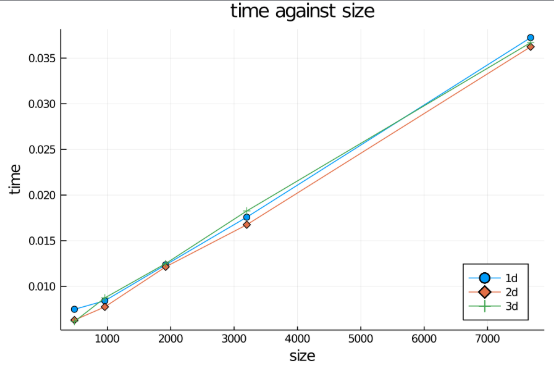
\includegraphics{lineartime.PNG}
  %\subfloat[$\epsilon_{\max}=5$]{\label{fig:a}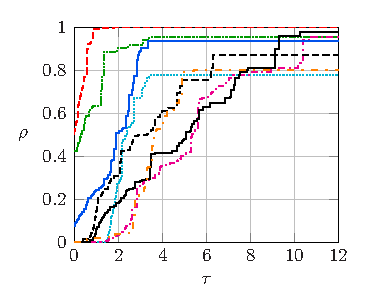
\includegraphics{lexample_fig1}}
  %\subfloat[$\epsilon_{\max}=0.5$]{\label{fig:b}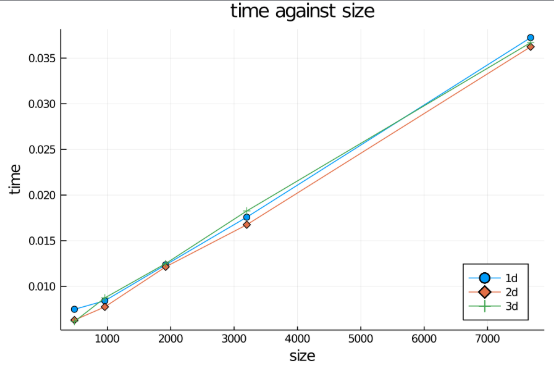
\includegraphics{lineartime.PNG}}
  \caption{time against size.}
  \label{fig:1}
\end{figure}
%\end{tcbverbatimwrite}
\subsubsection{Comparison with Ipopt package}
\begin{table}[H]
\caption{Comparison with Ipopt}
We run the experiments on the four cases in 1-dimensional setting with the size of 50, 100, 150, 200. The missing proportion is 0.05. The parameters for backtracking line search, Newton's method, and interior point methods are: $\epsilon_B = 10e-6, \mu_B = 10, \alpha_{LS} = 0.1, \gamma_{LS} = 0.8, \epsilon_{NT} = 10e-6.$
\begin{tabular}{|l|l|l|l|l|}
\hline
size                  & 50     & 100     & 150     & 200     \\ \hline
Interior point method & 0.0045 & 0.0471  & 0.0145  & 0.0182  \\ \hline
Ipopt                 & 2.3998 & 20.6119 & 133.557 & 463.951 \\ \hline
\end{tabular}
\end{table}
The Ipopt solver is much slower even when the size is small. This is partially because Ipopt solver cannot take advantage of the orthogonality in our problem.
\subsection{Accuracy}
Except for the time cost, we also care about how good is our estimate.
\subsubsection{MSE error}
Mean square error (MSE) is one metric to characterize the accuracy of the estimation. Denote the estimate of DFT as DFTest, then
\begin{equation}
    MSE = \frac{1}{n}\sum_{i=0}^{n-1} |DFT_i-DFTest_i|^2.
\end{equation}
Let $\mathcal{S} = \{i: DFT_i\neq 0\}$, then define
\begin{equation}
    MSE = \frac{1}{n}\sum_{i\in\mathcal{S}} |DFT_i-DFTest_i|^2.
\end{equation}
\begin{table}[H]
\caption{MSE of interior point method}
\begin{tabular}{|l|ll|ll|ll|}
\hline
Size & \multicolumn{2}{l|}{1 dim}                & \multicolumn{2}{l|}{2 dim}                & \multicolumn{2}{l|}{3 dim}                \\ \hline
     & \multicolumn{1}{l|}{MSE}    & MSE(sparse) & \multicolumn{1}{l|}{MSE}    & MSE(sparse) & \multicolumn{1}{l|}{MSE}    & MSE(sparse) \\ \hline
480  & \multicolumn{1}{l|}{0.1373} & 8.5865      & \multicolumn{1}{l|}{0.0414} & 3.6448      & \multicolumn{1}{l|}{0.1169} & 5.1326      \\ \hline
960  & \multicolumn{1}{l|}{0.0437} & 3.8637      & \multicolumn{1}{l|}{0.0463} & 9.6065      & \multicolumn{1}{l|}{0.0439} & 4.1085      \\ \hline
1920 & \multicolumn{1}{l|}{0.0378} & 9.1809      & \multicolumn{1}{l|}{0.0197} & 8.2287      & \multicolumn{1}{l|}{0.0262} & 4.8369      \\ \hline
3200 & \multicolumn{1}{l|}{0.0165} & 7.0304      & \multicolumn{1}{l|}{0.0065} & 4.2871      & \multicolumn{1}{l|}{0.0251} & 8.2055      \\ \hline
7680 & \multicolumn{1}{l|}{0.0088} & 8.9533      & \multicolumn{1}{l|}{0.0056} & 9.4672      & \multicolumn{1}{l|}{0.0098} & 8.0464      \\ \hline
\end{tabular}
\end{table}
\subsubsection{Sparsity identification}
Identifying the sparsity is our important goal. Thus, we take a look at how much nonzero entries we successfully discover. Here, ``true nnz" = the number of nonzero entries in DFT; "est nnz" = the number of nonzero entries in estimated DFT"; "recovery rate" = the proportion of true nnz discovered by this work.
\begin{table}[H]
\caption{Sparsity identification}
\begin{tabular}{|l|lll|lll|lll|}
\hline
Size & \multicolumn{3}{l|}{1 dim}                                                         & \multicolumn{3}{l|}{2 dim}                                                         & \multicolumn{3}{l|}{3 dim}                                                        \\ \hline
     & \multicolumn{1}{l|}{true nnz} & \multicolumn{1}{l|}{est nnz} & recovery rate & \multicolumn{1}{l|}{true nnz} & \multicolumn{1}{l|}{est nnz} & recovery rate & \multicolumn{1}{l|}{true nnz} & \multicolumn{1}{l|}{est nnz} & recovery rate \\ \hline
480  & \multicolumn{1}{l|}{6}        & \multicolumn{1}{l|}{104}     & 1.0                 & \multicolumn{1}{l|}{4}        & \multicolumn{1}{l|}{58}      & 1.0                 & \multicolumn{1}{l|}{8}        & \multicolumn{1}{l|}{92}      & 1.0                \\ \hline
960  & \multicolumn{1}{l|}{6}        & \multicolumn{1}{l|}{128}     & 1.0                 & \multicolumn{1}{l|}{4}        & \multicolumn{1}{l|}{60}      & 1.0                 & \multicolumn{1}{l|}{8}        & \multicolumn{1}{l|}{112}     & 1.0                \\ \hline
1920 & \multicolumn{1}{l|}{6}        & \multicolumn{1}{l|}{168}     & 1.0                 & \multicolumn{1}{l|}{4}        & \multicolumn{1}{l|}{68}      & 1.0                 & \multicolumn{1}{l|}{8}        & \multicolumn{1}{l|}{126}     & 1.0                \\ \hline
3200 & \multicolumn{1}{l|}{6}        & \multicolumn{1}{l|}{120}     & 1.0                 & \multicolumn{1}{l|}{4}        & \multicolumn{1}{l|}{68}      & 1.0                 & \multicolumn{1}{l|}{8}        & \multicolumn{1}{l|}{184}     & 1.0                \\ \hline
7680 & \multicolumn{1}{l|}{6}        & \multicolumn{1}{l|}{184}     & 1.0                 & \multicolumn{1}{l|}{4}        & \multicolumn{1}{l|}{60}      & 1.0                 & \multicolumn{1}{l|}{8}        & \multicolumn{1}{l|}{163}     & 1.0                \\ \hline
\end{tabular}
\end{table}
All the true nonzero entries are discovered, although the estimated nonzero entries are not very few. (I think this can be adjusted via revising the constraint threshold.)

\begin{table}[H]
\caption{Comparison with ADMM}
\begin{tabular}{|l|l|l|l|l|l|}
\hline
size                  & 480    & 960    & 1920   & 3200   & 7680   \\ \hline
Interior point method & 0.7285 & 1.0842 & 1.8639 & 2.3386 & 6.7089 \\ \hline
ADMM                  & 0.0065 & 0.4246 & 0.4955 & 1.7954 & 1.7954 \\ \hline
\end{tabular}
\end{table}
\section{Multidimensional spectral analysis with real datasets}\label{sec:real_datasets}
The pair distribution function analysis of powder samples (powder PDF) of crystals is a common tool for investigating disordered structures. The powder PDF is computed by the Fourier transform of the total X-ray or neutron powder diffraction pattern of a sample and provides a direct measure for the real interatomic distances in a material. PDFs from single crystals (3D-PDF) may be calculated by the Fourier transform either of the total single crystal diffraction pattern (total 3D-PDF) or of the diffuse scattering alone (3D-$\Delta$PDF). When the PDF is calculated in three dimensions, it is possible to remove the Bragg peaks before performing the transform by using a technique known as ``punch-and-fill", so that the resulting vector maps only
include those whose probabilities that differ from the average structure. This allows the disorder to be directly visualized without extensive modeling and vastly simplifies interpretation. The punch-and-fill algorithm involves the removal of Bragg peaks and ``fills" the data in the region of the Bragg peaks. The missing data at the Bragg peak locations are interpolated such that the missing data satisfies the 3-D Laplace difference equations. This has the following advantages  a) it results in a banded linear system of equations (tridiagonal for 1D, pentadiagonal for 2D and so on) sparse and hence one can leverage many sparse linear algebra techniques and software packages, b) another major advantage is instead of solving a single large linear system, one can solve smaller local linear systems corresponding to each Bragg peak and this operation is embarrassingly parallel. For example for a 3D volume data with 125M pixels (500 $\times$ 500 $\times$ 500) -- instead of solving a large 125M by 125M linear system, one can solve 1000 10K by 10K linear systems in parallel. However, the “punch-and-fill” algorithm (PFA) can generate unintentional ripples, or noise, in the resulting 3D-$\Delta$PDF because of sharp edges in the data interpolation. In order to mitigate this noise, we propose to exploit the fact that the 3D-$\Delta$PDFs should be inherently sparse, i.e., the PDF is essentially zero except for some discrete features encoding pairwise interatomic vector probabilities. The sparse DFT sparse recovery algorithm via the $l_1$ constraint minimization problem is ideally suited to this application. Figure \ref{fig:VO2}
\begin{figure}
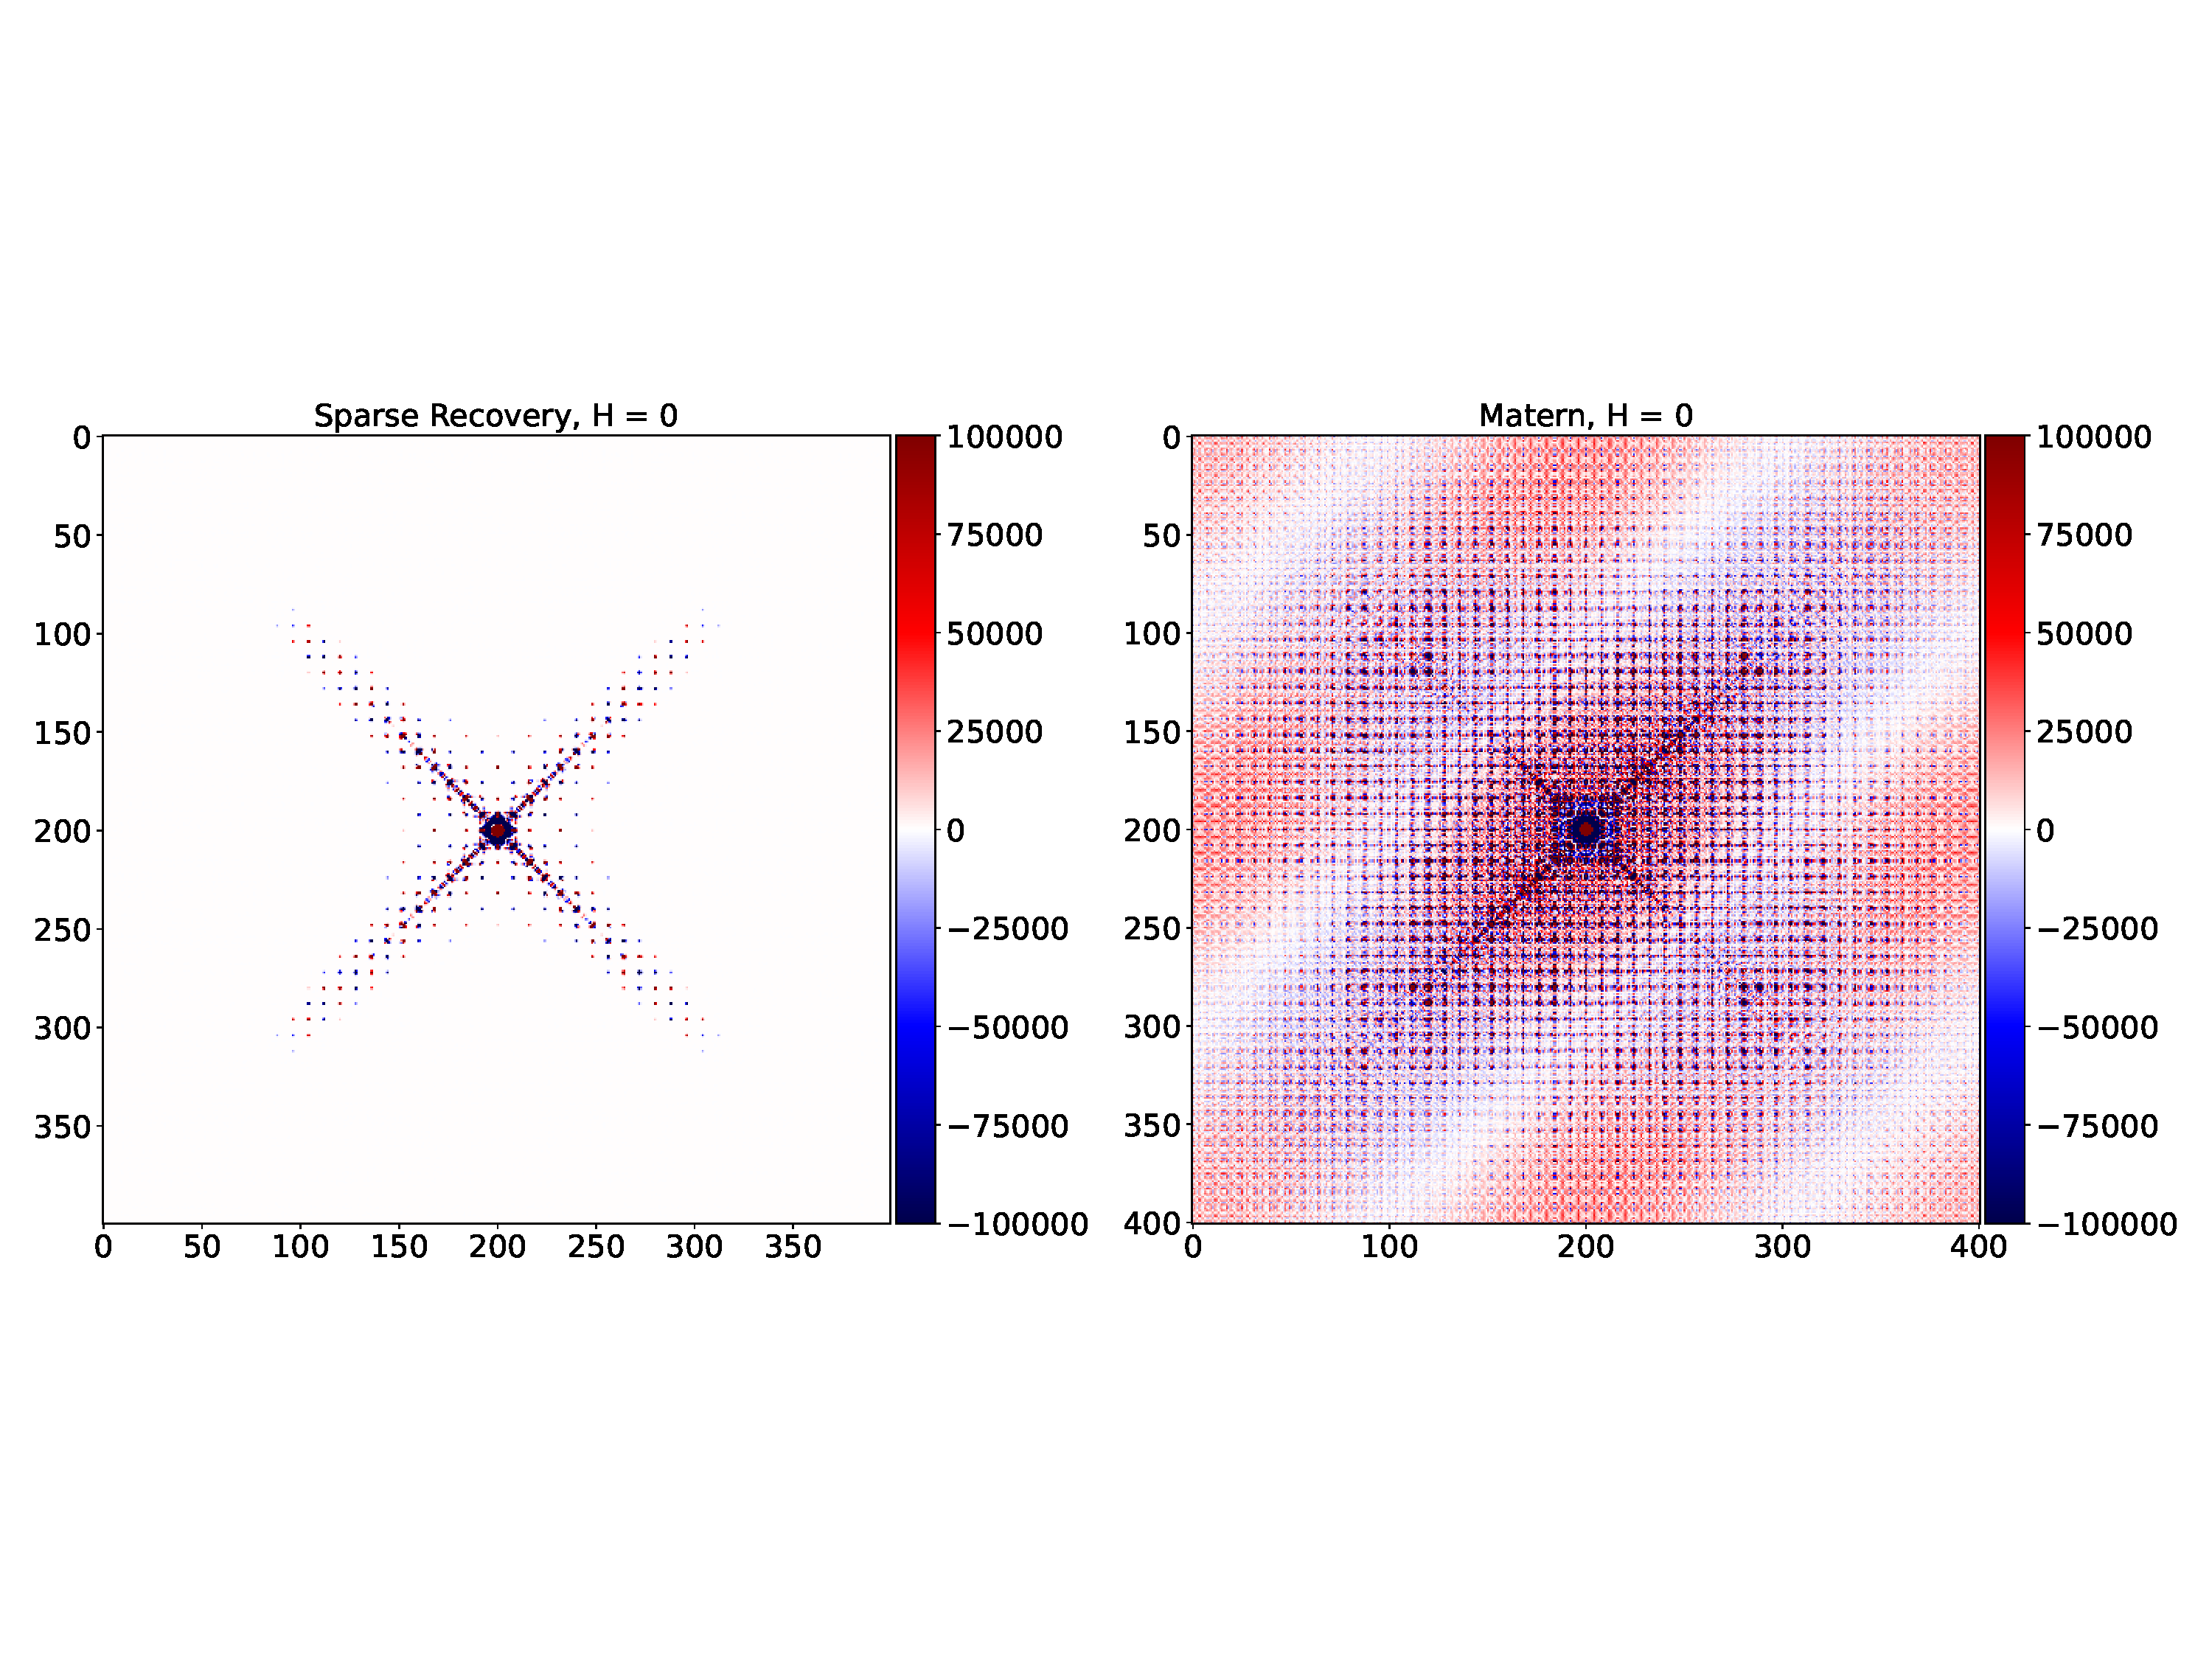
\includegraphics[width=\textwidth, trim=0in 4in 0in 4in 0in]{MaternVsSparse.pdf}
\caption{\label{fig:VO2} Left panel shows the sparse recovery, right panel shows ordinary punch and fill}
\end{figure}

\subsection{Large Scale Linear Algebra and Optimization for Data-Intensive Calculations}

% \subsection{Laplace Interpolation} \label{ss:laplace}
% The punch-and-fill algorithm is the most expensive computational step in computing the 3D-$\Delta$PDF in the standard workflow. The punch-and-fill algorithm involves the removal of Bragg peaks and ``fills" the data in the region of the Bragg peaks. Previously, the Bragg peaks were filtered by convolving with Gaussian smoothing operator. The Gaussian Smoothing Operator performs a weighted average of surrounding pixels based on the Gaussian distribution. While this approach filtered Bragg peaks well, it is computationally expensive ($\mathcal{O}(n^3 \log(k))$, where $n\times n \times n $ is the size of the volume data and the size of the Gaussian kernel is $k \times k \times k$). The smoothing using Gaussian Kernels has to performed using the entire dataset and does not easily lend itself for parallelization. 

% To overcome this computational limitation, we developed a linear interpolation technique such that the missing data satisfies the 3-D Laplace difference equations. This has the following advantages: a) it results in a banded linear system of equations (tridiagonal for 1D, pentadiagonal for 2D and so on) sparse and hence one can leverage many sparse linear algebra techniques and software packages, b) another major advantage is instead of solving a single large linear system, one can solve smaller local linear systems corresponding to each Bragg peak and this operation is embarrassingly parallel. For example for a 3D volume data with 125M pixels (500 $\times$ 500 $\times$ 500) -- instead of solving a large 125M by 125M linear system, one can solve 1000 10K by 10K linear systems in parallel. This results in great computational savings (for the 3D VO$_2$ data, we observed a six- to ten-fold reduction in compute time. This can be further enhanced by using parallel computing resources). Figure \ref{fig:punch_and_fill} shows a 1-D slice of the results of punch and fill using the Laplace interpolation on the VO$_2$ dataset. One notes that the performance of the new method is broadly comparable to the old one, but it is \textit{much faster}. The Laplace interpolation and a generalization of the Laplace interpolation -- called the Matern interpolation has been published as a Julia package (\texttt{LaplaceInterpolation.jl}) and more details about the package can be found in our paper \cite{RH2022}.

% \begin{figure}
%      \centering
%      \begin{subfigure}[b]{0.45\textwidth}
%          \centering
%          \includegraphics[width=\textwidth]{BraggPeaks.png}
%          \caption{1-D slice with Bragg Peaks}
%          \label{fig:BraggPeaks}
%      \end{subfigure}
%      \hfill
%      \begin{subfigure}[b]{0.45\textwidth}
%          \centering
%          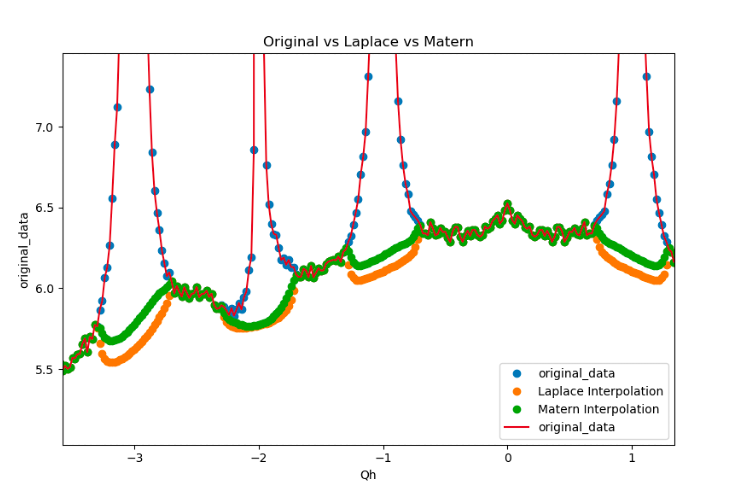
\includegraphics[width=\textwidth]{Punch_Fill.png}
%          \caption{1-D slice after punch-and-fill}
%          \label{fig:punch_fill}
%      \end{subfigure}
%         \caption{1-D slice with punch-and-fill using both Laplace and Matern Interpolation}
%         \label{fig:punch_and_fill}
% \end{figure}
% \begin{figure}
% 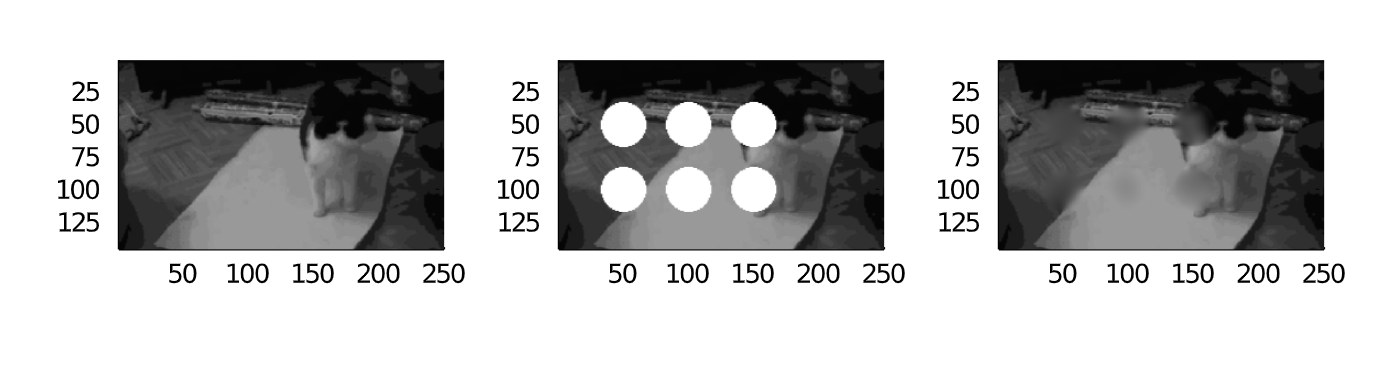
\includegraphics[width=\textwidth, trim=0in 4in 0in 4in 0in]{Figures/LaplaceInterp_3D.png}
% \caption{\label{fig:punch_and_fill} Left panel shows the original data, the center panel shows the right panel shows the data after punch and right frame shows the data after fill}
% \end{figure}
\subsection{Compressed sensing}

\begin{figure}
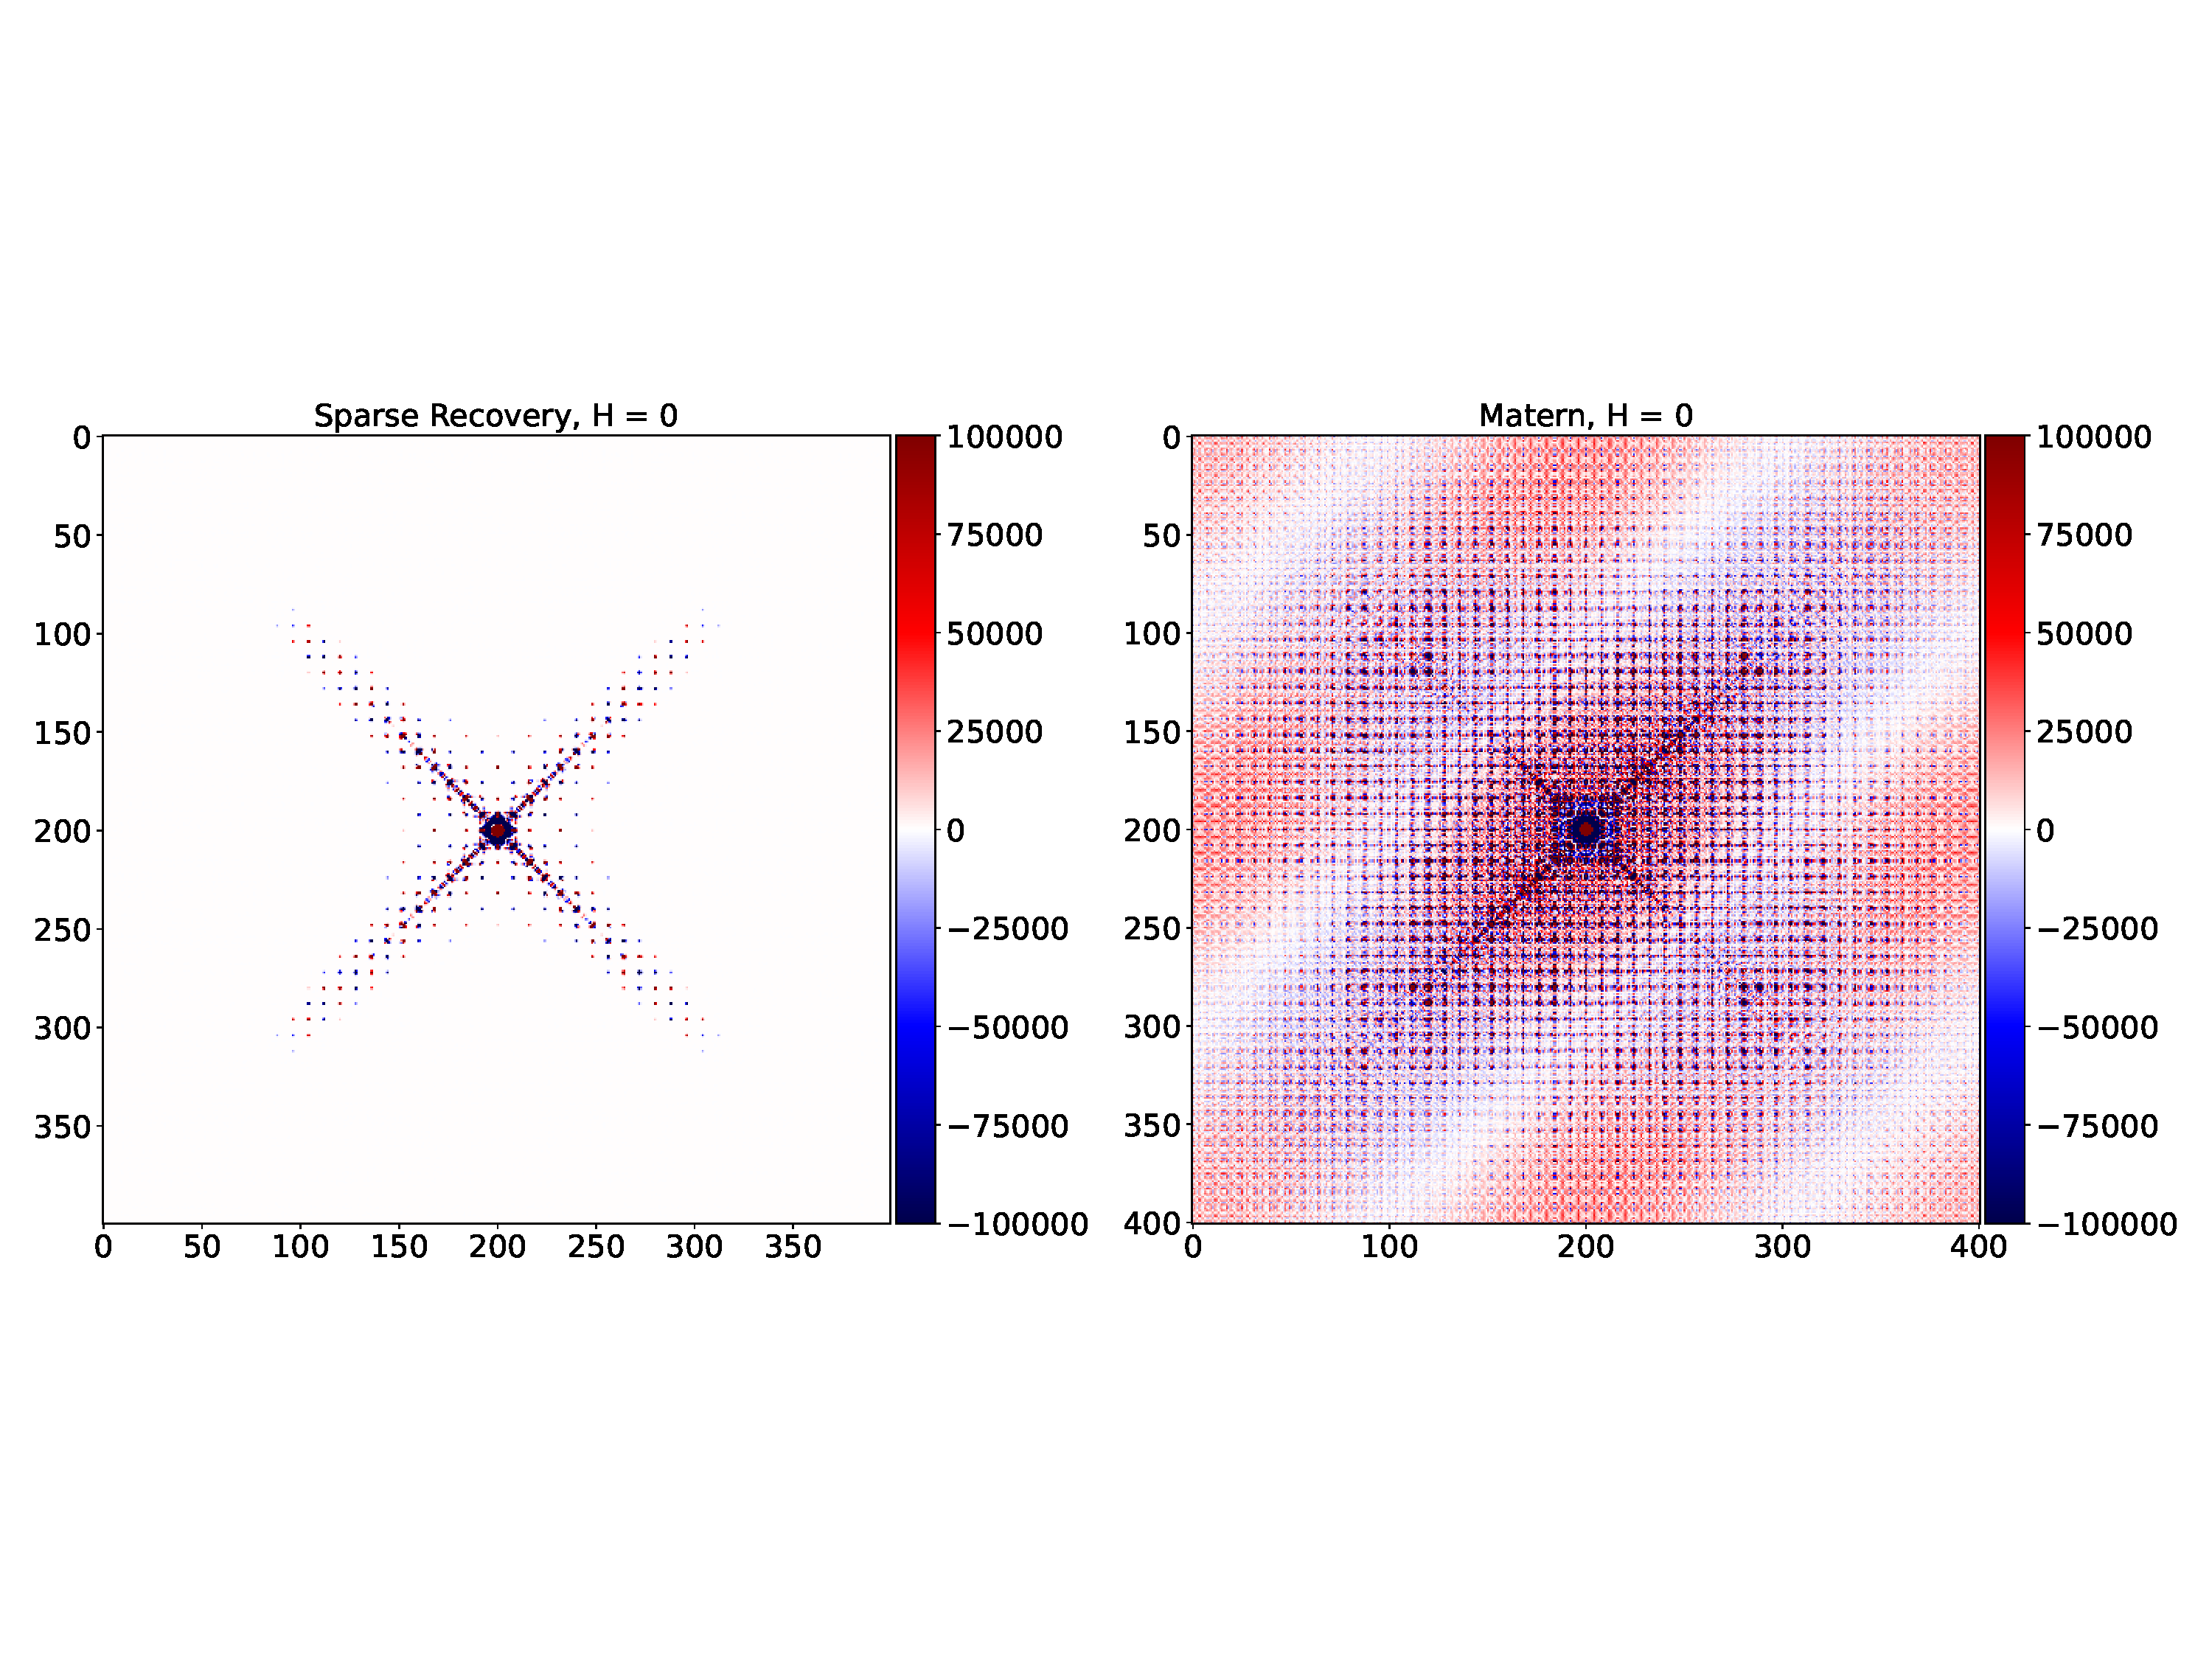
\includegraphics[width=\textwidth, trim=0in 4in 0in 4in 0in]{MaternVsSparse.pdf}
\caption{\label{fig:VO2} Left panel shows the sparse recovery, right panel shows ordinary punch and fill}
\end{figure}

Mathematically relevant to the study of the 3D-$\Delta$PDF is the notion that the
solution to the problem is inherently sparse, i.e. the PDF is essentially zero except
for some discrete features encoding pairwise interatomic vector probabilities
representing disorder in the crystal structure. Earlier approaches to this problem
involved removal of Bragg peaks using a punch-and-fill algorithm (including some
novel innovations of our own such as the \texttt{LaplaceInterpolation.jl} package, \cite{RH2022}) however the sharp edges
sometimes caused by the data interpolation could cause relatively large unintentional
ripples, or noise, in the resulting pdf. In order to mitigate this noise, we propose
a compressed sensing approach to solve the mathematical optimization problem which is characterized by an l1
constraint minimization. The punch-and-fill algorithm can be formulated as a problem of identifying the sparsity of Discrete Fourier transform (DFT) when the signal is noisy. Consider the noisy signal
\begin{equation}
    \widetilde{z} = \widetilde{x} + \widetilde{e}\,,
\end{equation}
we are in particular interested in the case where signal has some missing values, which intends to model the punching removal. Suppose the missing indices are recorded in a set $\mathcal{M}$. For simplicity, we denote our observed signal as
\begin{equation}
    z:=\widetilde{z}_{[n]\backslash\mathcal{M}},
\end{equation}
which are the observed values in the noisy signal. Then the loss function to minimize turns into $.$. 

Here we use the important insight that $v$ is sparse for many cases of interest. This can be mathematically enforced by adding an  $l_1$ constraint. Thus the resulting optimization problem becomes
\begin{equation}\label{eqn:complexopt}
    v = \arg\min_{v\in\mathcal{F}}\left\|z - \left(IFT(v)\right)_{[n]\backslash\mathcal{M}}\right\|_2 \text{ s.t. }\|v\|_1 \leq d,
\end{equation}
where the parameter $d$ characterize the sparsity of $v$. Alternatively, we can impose the sparsity constraint by using Lagrange multiplier, note that the objective is convex. We solve the above $l_1$ optimization problem using the alternating direction method of multipliers (ADMM)  approach and Figure \ref{fig:VO2} compares the results from interpolation and the compressed sensing approach. The left panel of the figure shows
the pdf using the compressed sensing algorithm (state parameters tuned here) in
comparison with the pdf calculated using the punch and fill algorithm, observe the vastly improved reconstruction. The reduction
of the low-profile noise to zero is the key advantage of the l1 minimization -
effectively reducing the complex features of the result to an interpretable set of
discrete interatomic vector probabilities. 

\subsection{An ADMM algorithm} The mapping $\left(IFT(v)\right)_{[n]\backslash\mathcal{M}}$ is a linear one in $v$ in problem \eqref{eqn:complexopt}. Therefore, by using the Lagrange multiplier approach to enforce the constraint of \eqref{eqn:complexopt} and replacing the objective using the classical notation $Ax=b$ for the underlying underdetermined linear system, and squaring the objective, the problem \eqref{eqn:complexopt} can be rephrased as 
\begin{equation} \label{}
    \text { minimize }(1 / 2)\|A x-b\|_{2}^{2}+\lambda\|x\|_{1}.
\end{equation}
To solve this convex nonsmooth optimization problem we use the alternating direction method of multipliers (ADMM). 
To start, we use a new variable and a penalty to state the equivalent problem
\begin{equation}
    \min_{x, z}(1 / 2)\|A x-b\|_{2}^{2}+\lambda\|z\|_{1} + \frac{\rho}{2}\|x-z\|^2,\text{ s.t. }x - z = 0.
\end{equation}
Since $\frac{\rho}{2}\|x-z\|^2$ is zero under the constraint $x - z = 0$ the two problems are identical. Using now a new Lagrange term for the constraint, we obtain
\begin{equation}
    \min_{x,z}\max_{y} L_{\rho}(x,z,y) = (1 / 2)\|A x-b\|_{2}^{2}+\lambda\|z\|_{1} + \frac{\rho}{2}\|x-z\|^2 + y^{\top}(x-z).
\end{equation}
The ADMM algorithm alternatively seeks the best objective by updating one variable at a time. 
\begin{equation}
    \begin{aligned}
x^{k+1} &:=\left(A^{T} A+\rho I\right)^{-1}\left(A^{T} b+\rho z^{k}-y^{k}\right) \\
z^{k+1} &:=S_{\lambda / \rho}\left(x^{k+1}+y^{k} / \rho\right) \\
y^{k+1} &:=y^{k}+\rho\left(x^{k+1}-z^{k+1}\right)
\end{aligned}
\end{equation}
where we have introduced the soft thresholding operator
\begin{equation}
S_{a}(x) = \begin{cases}x-a & x > a \\ 0 & -a\leq x\leq a\\ x+a & x<-a\end{cases}   \text{ for }a>0
\end{equation}
For problems of the size we are interested in, the first step is by far the most expensive. Since $A$ has orthogonal rows, we could use for the example we presented Sherman Morrison to reduce the computation to solving linear systems with matrices of the size of the few missing entries.  
However, for the larger problems we want to pursue here, we need even faster methods which underpins our proposed research. 







%\new{\textbf{Summary}}

%\new{\textbf{What we have done:} \begin{itemize}
%    \item Laplace Interpolation package for full 3D Volume dataset (this has been incorporated into the workflow).
%    \item Compressed sensing approach using ADMM for the full 3D Volume dataset (Vo2 data)
%\end{itemize}}

%\new{\textbf{What we plan to do:}  \begin{itemize}
%    \item Develop/Incorporate second order methods for the compressed sensing to accelerate the convergence of the optimization.
%    \item Accelerate the linear algebra components involved in the compressed sensing approach (Matrix-free methods, iterative methods, parallelism to take advantage of the dense structure etc.)
%\end{itemize}}


% The conjugate structure of DFT makes the optimization in complex field difficult. However, this can be reformulated as a LASSO in real field. Multiple first order and second order methods can be applied to solve the problem Besides, the orthogonal structure of inverse Discrete Fourier transform (IDFT) allows us to greatly reduced the storage. Also the operations of computing Newton direction is linear in problem size. Thus, our method is practical and scalable. 
% While such datasets can comprise over 100M pixels, the
% sparse recovery algorithm must be computationally efficient to be useful. This is the
% case for the Vo2 dataset pictured in the figure. The left panel of the figure shows
% the pdf using the compressed sensing algorithm (state parameters tuned here) in
% comparison with the pdf calculated using the punch and fill algorithm. The reduction
% of the low-profile noise to zero is the key advantage of the l1 minimization -
% effectively reducing the complex features of the result to an interpretable set of
% discrete interatomic vector probabilities. 
% This work was computed in collaboration with Wei Kuang, University of Chicago. 

% Compressed sensing is done by many people but it is not clear that they do it with
% enhanced computational speed. Nobody else has a second order method, etc. etc.
% Descriptors that explain what we are doing differently.



\section{Conclusion and future work}\label{sec:conclusions} In summary, this paper introduce how to apply interior point method to recover sparse DFT when the signal is noisy and has some missing values. The goal is achieved by transferring the optimization problem to LASSO. Beyond that, the storage is linear in $n$ as a result of the orthogonality of $A$. Also the orthogonality also allows us to do operations linear in $n$ when we find the Newton direction. These two factors make our method scalable.

Although we save tons of storage by only storing $M$, the size of $M$ is still too huge to store when problem size is too large. Fortunately, the missing values in crystal X-ray image have periodic structure, and the rows of $M$ share some similarity when they are around the same location. This possibly allows us to save only part of the missing rows and do interpolation to construct the rest, which is left as future work.

\bibliographystyle{siamplain}
\bibliography{references}

\end{document}
